
\tjzspis{Inteligentna metoda na cukier} %tytuł do spisu treści
\tjztyt{Inteligentna metoda na cukier} %tytuł odcinka

Bohaterami tej historii są: dociekliwy chirurg i~student, profesor będący z~nimi w~konflikcie, dziesiątki psów,  awantura o~Nobla, miliony świń i~krów, bakterie produkujące ludzkie białko, aż wreszcie inteligentne białko NNC2215, które daje nadzieję na dobre życie osobom dotkniętym śmiertelnie niebezpieczną chorobą, cukrzycą.

Myślę o~tym, wpatrując się w~karnawałowy rodzinny przysmak: kulkę z~orzechów zmieszanych z~koglem-moglem oblaną kruchym, połyskliwym karmelem. I~wyobrażam sobie, co się stanie, kiedy pokusa zwycięży rozum.

Strawiona słodycz doprowadzi do gwałtownego wzrostu stężenia glukozy we krwi. W~trzustce, a~dokładniej w~komórkach beta, tworzących tzw. wyspy, wzrost glukozy we krwi wywoła kaskadę reakcji ilościowo zależną od stężenia cukru. Maleńkie pęcherzyki znajdujące się tuż pod błoną komórkową uwolnią na zewnątrz hormon: insulinę. Im więcej cukru, tym więcej insuliny trafi do krwi. Rozprowadzana po całym ciele, zwiąże się z~cząsteczkami glukozy i~„zadokuje” do receptorów na powierzchni komórek, szczególnie komórek mięśni, tłuszczu i~wątroby. Połączone z~insuliną receptory zmienią swój kształt, dzięki czemu w~kaskadzie reakcji w~błonie pojawią się kanały wpuszczające glukozę do środka i~jej poziom we krwi obniży się.

Ten system ścisłej regulacji stężenia cukru we krwi  jest ważniejszy, niż by się zdawało. Glukoza jest „pokarmem” dla komórek – dzięki niej powstają cząsteczki ATP biorące udział we wszystkich reakcjach chemicznych wymagających wkładu energii. Z~drugiej strony pozostająca we krwi glukoza w~wysokim stężeniu jest śmiertelnie niebezpieczna. W~bardzo wysokim stężeniu w~krótkim czasie może doprowadzić do śpiączki, a~nawet śmierci. W~przebiegu przewlekłym jest przyczyną stanów zapalnych, prowadzi do uszkodzenia niewielkich naczyń krwionośnych odżywiających wszystkie ważne organy naszego ciała, szczególnie serce, układ nerwowy i~mózg. Tracimy czucie, mamy osłabiony układ odpornościowy, wysiadają nam próbujące usunąć nadmiar cukru nerki, źle goją się rany, grozi martwica tkanek.

Tak działoby się, gdyby moja trzustka nie wytwarzała insuliny. Gdybym była chora na cukrzycę.

Pierwsze wzmianki o~tej chorobie prawdopodobnie pojawiają się w~papirusach egipskich z~XV wieku p.n.e. Mowa o~ludziach wydalających więcej moczu, niż są w~stanie wypić płynów.
% To skutek nieefektywnej pracy nerek, które próbują usunąć nadmiar cukru z~moczu.
To efekt wytężonej pracy nerek, które próbując usunąć nadmiar cukru z~krwi, produkują dużo moczu.
Przez wieki chorzy cierpieli męki: byli odwodnieni, stale niedożywieni i~słabi. Jedyną metodą, aby żyć, było głodzenie się. Liczne komplikacje prowadziły do pogarszania się stanu zdrowia, śpiączki, a~po jakimś czasie do śmierci.\marg{
\includegraphics{art/202502_kol10}}

Cukrzyca była uważana za dysfunkcję żołądka lub jelit aż do 1889~roku, kiedy odkryto, że psy, którym usunie się trzustkę, stają się od razu diabetykami.  Wtedy to rozpoczął się wyścig: kto pierwszy wyizoluje czynnik odpowiedzialny za metabolizm cukru we krwi. Przez ponad 30 lat poszukiwania były nieskuteczne. Dalsza historia to trochę szczęścia, masa prób i~błędów, ale i~solidnej pracy naukowej. Jesienią 1920 roku młody kanadyjski chirurg Frederick Banting, przygotowując się do wykładu dla studentów, zapisał: „Podwiązać przewody trzustkowe psa. Utrzymać psy przy życiu, aż pęcherzyki (produkujące enzymy trawienne) ulegną degeneracji, pozostawiając wysepki. Spróbować wyizolować ich wewnętrzną wydzielinę, sprawdzić, czy zmniejsza glikozurię”. Z~propozycją zawiłej procedury podwiązywania przewodów trzustki psom i~uzyskiwania z~dysfunkcyjnej trawiennie trzustki ekstraktów do leczenia chorych Banting zwrócił się do speca od metabolizmu węglowodanów, profesora Johna Macleoda. Profesor był sceptyczny wobec tej idei, powątpiewając szczególnie w~jakość pracy eksperymentalnej zupełnie niedoświadczonego w~tej kwestii lekarza. Uznał jednak, że udostępni mu przestrzeń laboratoryjną, psy do eksperymentów oraz chętnego do pomocy studenta.

\advance\baselineskip by.1pt
Po kilku miesiącach skomplikowanych procedur początkujący naukowcy uzyskali bardzo niepewne wyniki, a~pierwotna idea izolacji poszukiwanego związku z~uszkodzonych trzustek psów została porzucona. Lepszym źródłem ekstraktu do badań okazały się mrożone trzustki krów i~świń, a~pierwsze testy na umierającym z~powodu cukrzycy dziecku dały spektakularny efekt: objawy po podaniu ekstraktu ustąpiły, choć natychmiast nastąpiła reakcja alergiczna.

Konieczne było bardzo staranne oczyszczenie preparatów, co wykonał znakomity chemik, James Collip. W~1921 roku czysty preparat zawierał substancję, którą nazwano insulina, od łacińskiego {\em insula} (wyspa). Po dwóch latach preparaty insuliny były już produkowane na masową skalę, a~Bantingowi i~Macleodowi przyznano za to odkrycie Nagrodę Nobla. Pominięto przy tym nie tylko Charlesa Benta, studenta, z~którym Banting robił wszystkie swoje doświadczenia, ale także Jamesa Collipa. Sprawa ta obróciła laureatów nagrody – a~z~nimi rzeszę ich popleczników – przeciwko sobie. Banting uważał, że Nobel należał się Bentowi, a~Macleod – że Collipowi. Na szczęście skandal naukowy nie wstrzymał dalszych badań.\marg{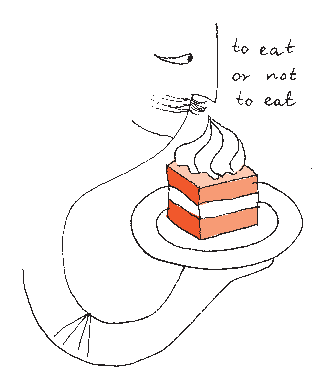
\includegraphics{art/202502_kol11}}

\vspace*{\parskip}
\begin{dwieszpalty}
Sekwencję insuliny ludzkiej opisano w~1953 roku (kolejna Nagroda Nobla), w~1963 roku zsyntetyzowano chemicznie, a~w~1969 określono strukturę przestrzenną cząsteczki. Okazała się peptydem – czyli niewielkim białkiem. Składa się z~21-aminokwasowego łańcucha~A i~30-aminokwasowego łańcucha~B, połączonych ze sobą dwoma wiązaniami. Badania nad mechanizmem działania insuliny – receptorami, z~którym się wiąże na powierzchni komórek, sposobem syntezy (wieloetapowej, mimo prostoty samej cząsteczki), kaskadami reakcji, które uruchamiają system regulacji stężenia glukozy we krwi, stworzyły rosnące pole do popisu dla nowych pomysłów, jak pomóc chorym na cukrzycę.

Jednym z~większych wyzwań była skala zapotrzebowania na lek. Pod koniec lat 70. XX~w. fabryka firmy Eli Lilly produkowała insulinę ze świńskich i~bydlęcych trzustek. Aby pokryć zapotrzebowanie w~USA, potrzeba było trzustek z~56~milionów zwierząt rocznie.  Konieczność odkrycia alternatywnej metody stała się priorytetem, szczególnie że odzwierzęcy lek powodował efekty uboczne.

Była to era gwałtownego rozwoju inżynierii genetycznej. W~roku 1978 udało się stworzyć  modyfikowane genetycznie bakterie syntetyzujące ludzką insulinę. Każdy z~łańcuchów peptydu był wytwarzany oddzielnie, izolowane z~bakterii łańcuchy były łączone w~całość w~laboratorium. Tę rekombinowaną insulinę podano pierwszym zdrowym ochotnikom w~1980 roku, a~rok później pierwszym chorym na cukrzycę.

Pomimo
% tych wszystkich sukcesów pacjenci dalej borykali się i~borykają nadal
tych sukcesów pacjenci do dziś borykają się
z~wieloma problemami. Konieczne jest stałe monitorowanie poziomu cukru i~dozowanie insuliny. Mimo zaawansowanej automatyzacji system regulacji poziomu cukru jest znacznie mniej precyzyjny niż naturalny. Na przykład insulina podawana przez skórę dociera do krwi z~opóźnieniem. Po posiłku stężenie glukozy jest czasowo za wysokie. Z~drugiej strony insulina stosunkowo długo się rozkłada, więc nie można podawać jej za dużo, bo zbyt duża ilość glukozy usuwana jest z~krwi, pozostawiając chorego w~stanie tzw. hipoglikemii, za~małego stężenia cukru. Zatem chory stale jest narażony na skoki poziomu cukru. To nie tylko szkodliwe dla organizmu, ale daje też szereg objawów utrudniających życie.

Dlatego już od 45 lat naukowcy próbują stworzyć „insulinę wrażliwą na glukozę” ({\em glucose responsive insulin}, GRI), która byłaby aktywna tylko wtedy, kiedy stężenie glukozy jest zbyt wysokie. Okazało się to trudne. Dopiero w~październiku zeszłego roku w~„Nature” zespół badaczy z~Danii opisał cząsteczkę NNC2215, która daje nadzieję, że cel jest blisko.

Do łańcucha B ludzkiej insuliny dodano dwa elementy. Z~jednego końca cząsteczkę, która przypomina glukozę (glukozyd), a~na drugim – związek makrocykliczny, czyli pierścień, do którego „pasuje” znajdujący się na drugim końcu NNC2215 glukozyd i~glukoza. Kiedy stężenie glukozy jest niewielkie, glukozyd przyłącza się do pierścienia, zaginając cząsteczkę tak, że nie pasuje do receptora insuliny, nie może zatem pełnić swojej funkcji. Kiedy glukozy jest więcej, wypiera glukozyd z~pierścienia, przez co NNC2215 się prostuje, co umożliwia jej połączenie się z~receptorem, a~w~konsekwencji otwarcie kanałów glukozy do wnętrza komórki. Stężenie cukru we krwi maleje, a~„inteligentna” insulina zwija się w~nieaktywną formę. Na razie NNC2215 przeszła testy na zwierzętach, w~tym na świniach, u~których cukrzyca i~mechanizm działania insuliny podobne są do ludzkich.  Czekamy na ciąg dalszy.

Nawet krótki wgląd w~aktualną wiedzę na temat cukrzycy jest jednoznaczny także dla zdrowych. Nadmiar cukru we krwi jest szkodliwy. Silna reakcja układu immunologicznego powoduje chroniczne stany zapalne, a~po tym lawinę skutków kończących się dysfunkcją wielu narządów, w~tym tych najważniejszych: serca, wątroby i~mózgu.  Wszyscy szczęśliwcy, których nie dotknęła cukrzyca, nie muszą polegać na inteligencji peptydów. Mogą użyć własnej… i~nie jeść cukrów. Nawet w~karnawale. 


%\eject

\medskip
\rightline{\large\it Marta FIKUS-KRYŃSKA}

\end{dwieszpalty}

\normalsize